This paper is inspired by the study of the Bitcoin transactions network performed by \cite{lischke2016analyzing}.
There, the authors examine the data for the first 4 years of the cryptocurrency with a goal of gaining insights about the underlying economy and its evolution.
They also apply a set of network metrics to identify major nodes, clusters, and verify whether the small world phenomenon exists for the Bitcoin network.

\begin{figure*}[ht]
  \centering
  \begin{subfigure}[b]{0.49\linewidth}
    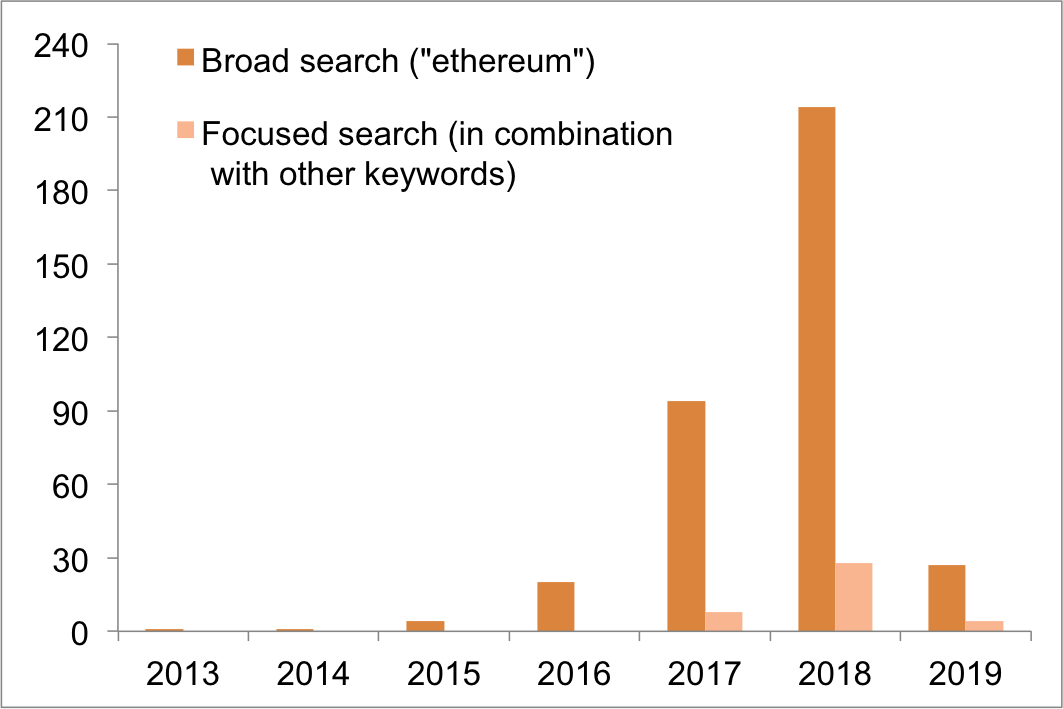
\includegraphics[width=\linewidth]{figures/search.png}
    \caption{Broad and narrow search for articles.}
    \label{fig:search_types}
  \end{subfigure}
  \begin{subfigure}[b]{0.49\linewidth}
    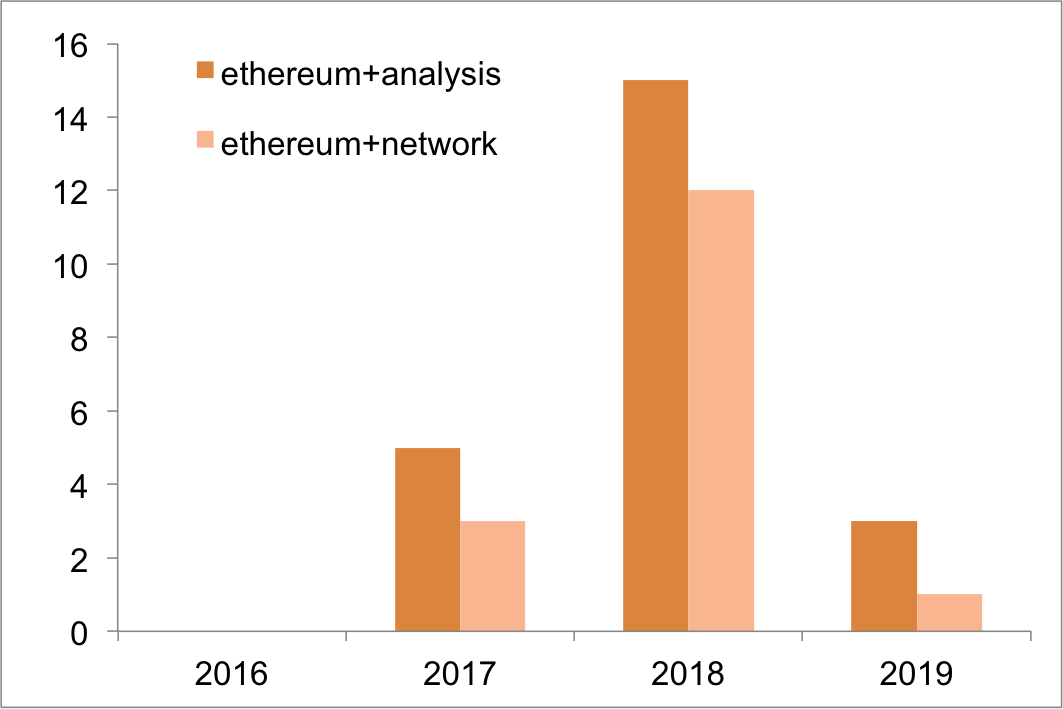
\includegraphics[width=\linewidth]{figures/narrow_search.png}
    \caption{Articles with a combination of keywords in the title.}
    \label{fig:narrow_search}
  \end{subfigure}
  \caption{Results of Google Scholar search for articles.}
  \label{fig:search}
\end{figure*}

The main distinctive feature of our research is that it targets Ethereum blockchain.
We replicate some of the approaches suggested in \cite{lischke2016analyzing} and adopt the others or come up with new approaches due to the differences in design and supporting infrastructure of the the cryptocurrencies.
Further details can be found in the Methodology section.

To make our analysis grounded on the previous Ethereum research, to benefit from findings and approaches described by other authors, to have an opportunity to compare our findings to previously obtained results and potentially to identify blank spots in the previous studies we conduct a literature review. 
As Ethereum was introduced only in 2013 the literature landscape is relatively scarce.
Most information is not peer-reviewed and is published on various blog-platforms, forums and wiki-resources.
This does not necessarily imply poor quality.
However, we decided to use those publications only as a source of background information.
Instead, the focus was made on publications that can be found using Google Scholar web search engine that indexes the full-text scholarly literature.

% In the first place we made an attempt to perform a quantitative analysis of the literature landscape.
We identified 361 articles that are published in the period from January 2013 till March 2019 and have the keyword "ethereum" in their title. 
For comparison, the search for articles published in the same time range but with keywords "cryptocurrencies", "bitcoin" and "blockchain" returns 618, 3670 and 6540 results respectively.
Figure \ref{fig:search_types} shows the dynamics in the number of publications that target Ethereum. 
Results for both broad and narrow (in combination with other keywords) searches are presented.
There is considerable growth over the last years.
% Nevertheless, the percentage of articles that are aimed at the Ethereum blockchain analysis is limited.
Nevertheless, only 11 \% of articles are aimed at the Ethereum blockchain analysis.
Thus, using a combination of the keyword "ethereum" with keywords "analysis" and "network" we identified 23 and 16 publications respectively (see Figure \ref{fig:narrow_search}).
Using other keywords such as "description", "graph", etc. provided only 1 additional article. 


Our literature review is based on (but not limited to) these articles.
At the later stage, we excluded part of them due to being out of immediate scope - excluded articles were dedicated to the analysis of price fluctuations, private implementations of Ethereum blockchain, new utility tokens or blockchain applications, social infrastructure around the Ethereum blockchain (like meetups or forums for blockchain discussions), etc.
More publications were identified when studying the initial set of articles and by screening the search results for broader keywords such as "ethereum" or "cryptocurrencies".

Most of the literature corpus relevant to the topic of Ethereum blockchain analysis can be grouped in 4 broad categories: (i) data collection, (ii) descriptive analysis, (iii) network metrics and graph analysis, (iv) smart contracts.
% (iii) activity, network components, graph analysis, descriptive analysis, network analysis, 

\textit{Data collection.} Certain part of the literature corpus is dedicated to the ways how Ethereum blockchain data can be gathered and aggregated for the sake of future analysis. For instance, 
\cite{li2017etherql} develop a query layer that allows collecting various data about blocks and transactions, as well as calculating balances of accounts.
\cite{pratama2018query} come up with similar query functionalities.
They facilitate access to blockchain data based on multiple search parameters (retrieval query), provide simple statistical analysis (aggregate query) and sort data according to its various components (ranking query).
\cite{perezanalysis} analyzes different node client software and APIs that can be used to access blockchain data.
He develops a tool that serves as an interface between the blockchain data and data analysis packages in Python.



\textit{Descriptive Analysis.} A number of publications perform descriptive analysis of the Ethereum blockchain.
Thus, \cite{payette2017characterizing} research Ethereum address space. 
Using the k-means clustering algorithm and other techniques, they identify 4 distinct groups of addresses, evaluate them quantitatively and qualitatively.
They show that clusters differ significantly in terms of the volume and amount of ingoing and outgoing transactions.
The authors also suggest that analysis of the amount of gas spent is crucial in "determining whether Ethereum is being utilized as a distributed supercomputer as intended by its creators or a vehicle for financial speculation".
\cite{anoaica2018quantitative} perform quantitative description of activity on the Ethereum blockchain. 
They 
% evaluate whether the network is robust against attacks, 
estimate the distribution of internal activity among users, identify most active addresses.
According to the authors, only 3 \% of nodes have participated in more than 10 transactions, while smart contracts account for only 9,5 \% of monetary value transfers.
% With regard to the network robustness to isolated attacks they conclude that power law distribution of nodes degree lies in the observed range for most real network.
\cite{kim2018measuring} also evaluate activity of the Ethereum nodes. 
They find out that less than half of all nodes contributes to the Ethereum Mainnet. 
A comparison with other P2P networks, such as BitTorrent or Bitcoin, reveals that Ethereum differs in both network size and geographical distribution. 
Ethereum is assessed as a small and immature P2P network that would benefit from the adoption of the known best practices.
The authors also identify network inefficiencies, such as outdated clients prone to patched vulnerabilities and hard fork incompatibility.

Descriptive analysis is done with the second goal of security assessment in several papers. 
For instance, \cite{kiffer2017stick} research the Ethereum/Ethereum Classic hard-fork that happened in 2016. 
Based on the comparison of various descriptives, such as hash rate, difficulty per block, number of transactions, number of blocks won by the major mining pools, the number of rebroadcast transactions, etc. they show the impact of the fork on the two networks and their mining pools.
They suggest that the fork led to unintentional incentives and security vulnerabilities. 
For instance, there is a security vulnerability wherein attackers can rebroadcast transactions from one network into the other.
Ethereum Classic experienced a loss of almost 90 \% of the nodes in its network immediately after the fork which also exposed it to various types of attacks.

Sometimes analysis is accompanied by suggestions of possible improvements or of practical applications. 
So, \cite{bentkeanalysis} researches pending transactions and optimal acceptance criteria for them. 
The author shows that pending transactions are related to the problem of double spending attacks and issues with the network topology.
He suggests workarounds for these problems that are applicable in certain circumstances.  
\cite{dennis2019analysis} analyze historical data about Ethereum and Bitcoin networks. 
Based on this analysis they model the growth of these networks in the future and propose ways that can help to reduce the networks' size and increase their scalability.
\cite{signer2018gas} develops a tool to analyze and visualize gas costs and consumption.
The author suggests that his tool can be used to explore gas consumption before deployment of smart contracts, is useful for a more gas-efficient and secure development of them. 



\textit{Network metrics and Graph analysis}. Many articles are based on the network theory and apply specialized visualization tools in their research.
Thus, \cite{chen2018understanding} perform graph analysis in order to evaluate major activities on Ethereum blockchain: money transfer, smart contract creation, and smart contract invocation. 
For each type of activities they estimate network metrics such as degree distribution, clustering, degree correlation, node importance, etc. 
Based on a set of quantitative estimations the authors conclude that (i) Ethereum is used mainly for transactions, smart contracts are not adopted actively, (ii) many of the users don't use Ethereum frequently, (iii) a considerable number of smart contracts is created by a small number of developers, (iv) financial hubs, such as exchanges dominate Ethereum.
Besides, they showcase how graph analysis can be used (i) to detect abnormal and potentially malicious contract creation, (ii) to identify smart contracts and accounts controlled by the malicious developer.
\cite{chan2017Ethereum} suggest a model for collection and graph analysis of the Ethereum transactions through a graph database management system Neo4j. 
The authors collect from Etherscan block explorer a set of addresses that are known to be associated with hacks on currency exchanges Gatecoin and Coindash. 
Using the model they try to de-anonymize these addresses and find out that hacked money ended up at a set of cryptocurrency exchanges (Changelly, ShapeShift, Bitfinex, Bittrex, and Poloniex). 
The authors suggest that linking Ethereum and Bitcoin transaction graphs in order to follow the money further and potentially reveal identities of the hackers.

Network theory based articles usually evaluate power law distributions in Ethereum network.
For example, \cite{somin2018social} and \cite{somin2018network} study the dynamics of the ”social signals” of Ethereum network, provide insights about the ecosystem and the forces acting within it.
The authors estimete that the network displays strong power-law properties.
According to them, this is the case for degree distribution of nodes, but as well for distribution of token popularity, in terms of buyers and sellers amount.
\cite{anoaica2018quantitative} conduct similar research and conclude that the network is robust to isolated attacks as power law distribution of nodes degree lies in the range that is observed for most real networks.
\cite{zwang2018detecting} use network theory to detect bot activity on Ethereum Blockchain. 
They show that time difference between consecutive Ethereum transactions also follow the power law distribution.
Consequently, deviation from this distribution are helpful to identify non-human activity. 
 
 

\textit{Smart contracts}. Given the role that smart contracts play in Ethereum blockchain we also consider publications on this topic. 
For instance, \cite{bartoletti2017dissecting} research practical applications of smart contracts. 
They identify different categories of smart contracts such as "financial", "game", "wallet", "library", etc. and quantify their usage.
The authors also come up with a classification of the most common design patterns and relate them to application domain categories.
\cite{bistarelli2019analysis} analyze the code of the verified smart-contracts and compilers. 
They identify opcodes - functionalities that are of special practical importance - and perform a statistical research of them. 
Results are suggested to be used for optimization of the smart-contracts development.
\cite{bennink2018analysis} study how interaction between different Ethereum blockchains and tokens can be performed. 
They analyze atomic swaps - smart contracts that allow executing the cross-chain exchange of funds or single-chain exchange of different tokens in a decentralized fashion.
The authors design single-chain token swap contract as a proof of concept, suggest theoretical improvements for other forms of atomic swaps.

A number of authors suggest specialized tools for analysis of the smart contracts. 
For example, \cite{albert2018ethir} come up with a framework for decompilation of the EVM bytecode.
The framework can be useful when the source code is not available.
This is the case in many situations, for instance, gas consumption is specified at the level of EVM instructions.
The framework allows performing analysis of smart contracts, for example in order to infer their loop bounds.
\cite{grishchenkoethertrust} develop a tool for bytecode analysis that captures important security properties of smart contracts, such as the single entrance or the independence of the transaction environment, and helps to identify when these properties are violated.

The topic of security concerns is dominant in articles dedicated to smart contracts. 
Thus, \cite{grishchenko2018semantic} do semantic analysis of Ethereum smart contracts. 
They define security properties of smart contracts, such as call integrity, atomicity, independence of transaction environment, independence from miner controlled parameters, etc.
The authors identify mistakes and imperfections in existing semantics and verification tools for Ethereum smart contracts, suggest their improvement.
This research is further extended in \cite{grishchenko2018foundations}, where the authors overview the state-of-the-art in smart contract verification.
They compare different verification tools for automated bug-finding, verification of generic properties, semi-automated proofs for contract specific properties, dynamic monitoring for predefined security properties, etc.
\cite{tikhomirov2018smartcheck} come up with a classification of code issues in Solidity language used for the creation of smart-contracts. 
They also suggest a statistic tool that can help to detect these issues.
Based on the large corpus of smart contracts, the authors find out which of them are the most common and severe.
\cite{bartoletti2017dissecting} suggest ways to identify Ponzi schemes on Ethereum blockchain. 
The authors analyse their development and impact on participants and Ethereum blockchain from various viewpoints. 
According to the research, 10 \% of the studied 1384 contracts with verified source code
on etherscan.io are Ponzi schemes. 
Nevertheless, the impact of these smart contracts is limited, as they cover only 0.05 \% of the transactions on the Ethereum blockchain.


A meta-analysis of the articles shows that all 4 major categories are covered in a relatively equal way (see Figure \ref{fig:search_types}).
Data collection about the blockchain receives less attention of the specialized articles.
This seems to be justifiable, sice data collection is just the first step of the analysis and other articles usually also have some minor part dedicated to this process.
Most of the attention is given to smart contracts, which can be explained by the importance of this Ethereum blockchain feature.

\begin{figure}[h]
  \centering
  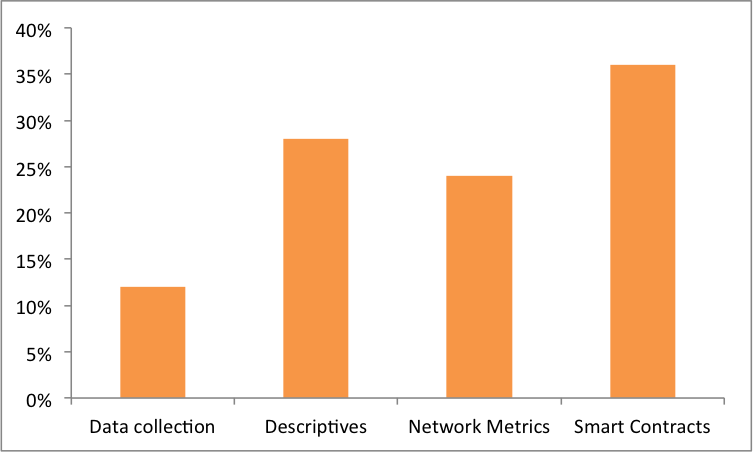
\includegraphics[width=\linewidth]{figures/literature.png}
  \caption{Literature Landscape.}
  \label{fig:literature}
\end{figure}

In our research, we will focus on descriptive and network metrics that are slightly less present in the current research landscape.
In conformity with the best practices set by reviewed papers, we will aspire to perform our analysis having in mind potential security and privacy issues that can be identified or inferred in the process.

To conclude the literature review section, we should add that a number of other articles that are not directly related to the analysis subject deserve the attention of those interested in future research on it. 
Thus, we have considered generic information about Ethereum: 
including its white and yellow papers (see \cite{buterin2014next} and \cite{wood2014Ethereum}) that describe technical specifications and design features of the blockchain; 
comparative studies of cryptocurrencies (see for instance \cite{maesa2018blockchain}, 
\cite{rudlang2017comparative}, 
\cite{sapuric2017distributed}, 
\cite{anderson2016new}) that allow to get a better understanding of the differences between Ethereum and Bitcoin blockchains and provide the necessary background for analysis and reasoning.

To complete the picture, we also considered research publications on network analysis of Bitcoin blockchain that are cited in \cite{lischke2016analyzing} and have provided us with some additional insights and inspiration: 
\cite{reid2013analysis}, 
\cite{baumann2014exploring}, 
\cite{drainville2012analysis}, 
\cite{ober2013structure}, 
\cite{meiklejohn2013fistful}, 
\cite{spagnuolo2014bitiodine}, 
\cite{androulaki2013evaluating}, 
\cite{kaminsky2011black}, 
\cite{ortega2013bitcoin}.






% \cite{greene2018investigation} perform an investigation into a denial of service attack on Ethereum blockchain.